\documentclass[letter,12pt]{article}


\usepackage[english]{babel}

\usepackage{fancyhdr}


\usepackage{graphicx}
\usepackage{amsmath}
\usepackage{amssymb}
\usepackage[latin1]{inputenc}
\usepackage{fancybox}
\usepackage{amsfonts}
\usepackage{bbold}
\usepackage{textcomp}


\setlength{\oddsidemargin}{0in}
\setlength{\evensidemargin}{0in}
\setlength{\textwidth}{16.1 cm}
\setlength{\topmargin}{-15mm}
\setlength{\textheight}{22cm}
\setlength{\parindent}{0cm}


\newcommand{\sv}{\underline}
\newcommand{\Sig}{\boldsymbol{\sigma}}
\newcommand{\K}{\boldsymbol{K}}
\newcommand{\Eps}{\boldsymbol{\varepsilon}}
\newcommand{\intener}{\mathcal{E}}


% --------------------------------------------------------------------------------------
% - definition des notations
% --------------------------------------------------------------------------------------


% - tenseur d'ordre 4
\newcommand{\TTTT}[1]{\underline{\underline{\underline{\underline{#1}}}}}
% - tenseur d'ordre 2
\newcommand{\TT}[1]{\underline{\underline{#1}}}
% - tenseur d'ordre 1
\newcommand{\T}[1]{\underline{#1}}

% - composante i - j de la contrainte: 
\newcommand{\sigi}[1]{\sigma_{#1}}
% - composante i - j de la deformation: 
\newcommand{\epsi}[1]{\varepsilon_{#1}}

% - tenseur de contrainte : 
\newcommand{\sig}{\TT{\sigma}}
\newcommand{\eps}{\TT{\varepsilon}}
\newcommand{\C}{\TTTT{C}}
\renewcommand{\S}{\TTTT{S}}

% - composantes des tenseurs de Hooke: 
\newcommand{\Ci}[1]{C_{#1}}
\newcommand{\Si}[1]{S_{#1}}

% - notations pour un vecteur
\renewcommand{\Vec}[1]{\underline{#1}}


% - notations pour un vecteur chapeau
\newcommand{\Vecc}[1]{\hat{\underline{#1}}}

% - notations pour un produit tensoriel
\newcommand{\tens}[2]{#1 \otimes #2}

% - notations pour les vecteurs de base
\newcommand{\e}[1]{\Vec{e_{#1}}}

% - contrainte equivalente pour les crit�res de plasticite
\newcommand{\se}{\sigma_{eq}}

% - deformation elastique
\newcommand{\epse}{\TT{\varepsilon_e}}

% - deformation elastique
\newcommand{\epsp}{\TT{\varepsilon_p}}


\begin{document}
\pagestyle{fancy}

\title{\textbf{Maximum shear stress}}
\date{}

\maketitle

\begin{figure}[h!]
\begin{center}
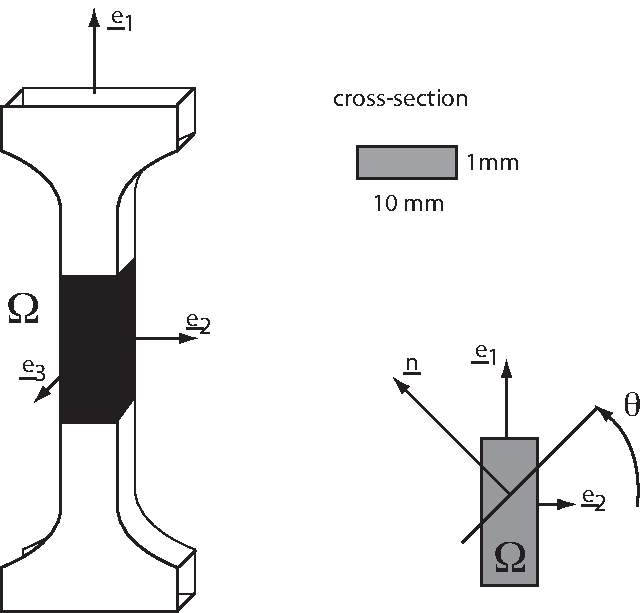
\includegraphics[width=0.4\columnwidth]{./exo2_traction}
\caption{Tensile test. We assume an homogeneous stress state within the central part of the sample.}\label{ex2}
\end{center}
\end{figure}


We assume that during a tensile test (figure \ref{ex2}), the stress state is homogeneous within the part $\Omega$ of a material sample. For any material point of $\Omega$, the local stress tensor is:


\begin{equation}
\sig  = 100 \cdot  \e{1} \otimes \e{1} 
\end{equation}

\begin{description}
\item{\textbf{Question 1}} Calculate the global force $\Vec{F}$ that is applied on the material sample by the experimental tensile device.
\item{\textbf{Question 2}} We cut the sample by a ``fictive" plane. The orientation of this plane is denoted by the angle $\theta$ between the $\Vec{e}_2$ axis and the unit normal vector $\Vec{n}$. Calculate as a function of $\theta$ the stress vector applied on this surface.
\item{\textbf{Question 3}} Find the value of $\theta$ for which the shear stress is maximum. 
\end{description}





\end{document}